\documentclass[preprint]{sigplanconf}
\usepackage{xspace,url,subfigure,framed,amssymb,
            amsmath,mathpartir,hyperref,
            stmaryrd, graphicx, fancyvrb, stmaryrd % double brackets llbracket
}

\usepackage[T1]{fontenc}
\usepackage{beramono}
\usepackage{listings}
\usepackage[usenames,dvipsnames]{xcolor}

\lstdefinelanguage{Julia}%
  {morekeywords={abstract,break,case,catch,const,continue,do,else,elseif,%
      end,export,false,for,function,immutable,import,importall,if,in,%
      macro,module,otherwise,quote,return,switch,true,try,type,typealias,%
      using,while},%
   sensitive=true,%
   morecomment=[l]\#,%
   morecomment=[n]{\#=}{=\#},%
   morestring=[s]{"}{"},%
   morestring=[m]{'}{'},%
}[keywords,comments,strings]%

\lstset{%\lstinputlisting[language=Octave]{BitXorMatrix.m}
    language         = Julia,
    basicstyle       = \small\ttfamily,
    keywordstyle     = \bfseries\color{blue},
    stringstyle      = \color{magenta},
    commentstyle     = \color{ForestGreen},
    showstringspaces = false,
    stepnumber=1,
    numbers=left
}

\newcommand{\rn}[1]{#1}
\newcommand{\doi}[1]{doi:~\href{http://dx.doi.org/#1}{\Hurl{#1}}}

\newcommand{\xt}[1]{\texttt{#1}}

\newcommand{\OK}[1]{#1\;\text{OK}}
\newcommand{\abstype}[2]{\xt{abstract}~#1 <: #2}
\newcommand{\oftype}[2]{#1\,::\,#2}
\newcommand{\m}[2]{{#1}(#2)}
\newcommand{\contype}[2]{\xt{type}~#1 <: #2}
\newcommand{\any}{\xt{any}}
\newcommand{\jolt}{\xt{JOLT}}

\newcommand{\exact}[1]{{\llbracket #1 \rrbracket_{\xt{exact}}}}
\newcommand{\usable}[1]{{\llbracket #1 \rrbracket_{\xt{}}}}
\renewcommand{\ldots}{...}
\newcommand{\cnum}[2]{$\text{#1}_#2$}


\conferenceinfo{NOOL '16}{Month d--d, 20yy, City, ST, Country} 
\copyrightyear{20yy}
\copyrightdata{978-1-nnnn-nnnn-n/yy/mm}
\copyrightdoi{nnnnnnn.nnnnnnn}
\begin{document}
\title{Bottom-up Objects - Static Typing Without Types} 
\authorinfo{Benjamin Chung \and Paley Li \and Jan Vitek}{Northeastern University}{bchung@ccs.neu.edu \and \{pa.li,j.vitek\}@neu.edu} % Annon : Benjamin Chung, Jan Vitek}{Northeastern University}{}
\maketitle
% We should probably have some more introductory/motivational material herezies

\begin{abstract}
TODO:
\begin{itemize}
\item Julia has interesting inheritance mechanism, but it's completely dynamic.
\item What we purpose: using statically type check to allow more complex inheritance structure and bring static error messages for inheritance structure to Julia.
\item We formalised our ideas in JOLT, a minimal subset of Julia.
\end{itemize}
\end{abstract}


\section{Introduction}

Traditional typed object-oriented languages have a series of
common idioms: single dispatch, to figure out which method
to use in which situation, interfaces, to abstract over 
common means of access, and the means to statically
ensure that those interfaces are adhered to.

These practices are perfectly suitable for many contexts,
as is demonstrated by the success of langauges that have 
these features, but are not universally applicable, and
other languages that do not have any of these features
can use the object abstraction while retaining static 
safety.

In this paper, we will be talking about the Julia
programming language. Julia was originally designed
as a scientific computing language, in the vein of 
R or Matlab, and has a number of features designed
to support numeric computation and other tasks common
in scientific work.

\begin{figure}[h]

\lstinputlisting[language=Julia]{broken.jl}
\begin{Verbatim}[fontsize=\small]
ERROR: MethodError: no method matching a(::C3)
Closest candidates are:
  a(::C1)
  a(::C2)
\end{Verbatim}
\caption{Object inheritance in Julia}
\label{code:broken}
\end{figure}


\begin{figure}
\centering
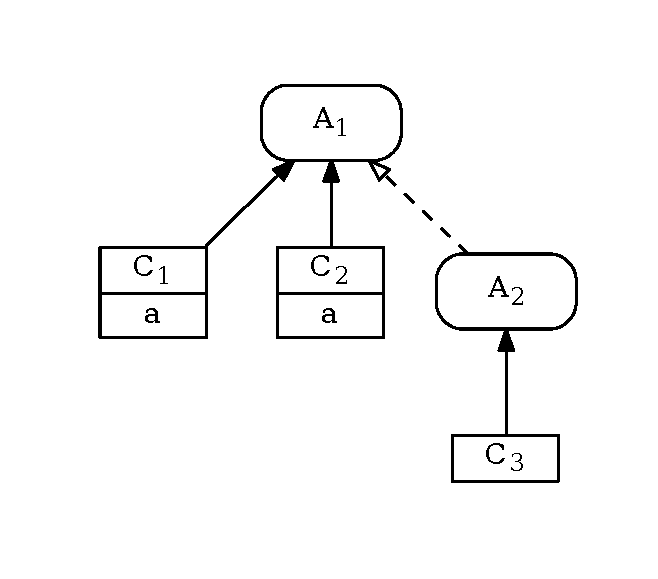
\includegraphics[scale=.6]{example2.pdf}
\caption{LALALALA}
\label{fig:algo}
\end{figure}

\section{Julia}

From the perspective of object systems, Julia has several interesting features:
\begin{itemize}
\item Julia is \emph{dynamically typed}, and has no mechanism for statically
checking type correctness. However, as illustrated in figure~\ref{code:broken},
Julia code has many types.
\item The reason for all of these types is \emph{dispatch}. Julia provides 
full multimethod dispatch based on \emph{runtime type tags}, letting programmers
write code that is highly specified for a specific value.
\item However, one of the odder properties of this system is that Julia does not
allow explicit procedural interfaces, one of the key features of traditional 
object systems. Instead, Julia's interfaces, called \emph{abstract types}, 
define no explicit methods, relying on ``a collection of informal interfaces''
\cite{juliadocu} to abstract over implementations.
\end{itemize}

Figure~\ref{code:broken} provides an illustration of how these features 
interact, and how they can be used to do untyped object-oriented programming.
The figure begins by constructing the object heirarchy shown in figure~
\ref{fig:algo}, then adds the method \xt{a} to the concrete classes $\text{C}_1$ and
$\text{C}_2$. The last function definition adds a function \xt{problem} to the
program, which calls the function \xt{a} on an argument of type $\text{A}_1$.

The next step is to actually call the methods we have defined. Julia performs
dispatch by looking for the \emph{most specific method} whose arguments are
satisfied by the given value - in essence, giving us a type guarantee that the
argument will always be of the declared type. In this way, the implementation 
of \xt{a} on line 7 is called when we call \xt{a} with an instance of $\text{C}_1$,
and the implementation of \xt{a} on line 8 is called for $\text{C}_2$.

However, the unchecked nature of Julia interfaces becomes apparent when we consider
$\text{A}_2$ and $\text{C}_3$. \cnum{C}{3} has no $\xt{a}$ implementation, and
therefore, despite being a subtype of \cnum{A}{1} 
(transitively, through \cnum{A}{2}), a call to \xt{a} with an instance of \cnum{C}{3}
fails with the error that no implementation of $\xt{a}$ exists for \cnum{C}{3}.

This problem is easy to spot in this example, because all of the type defintions
are simple and in the same place. However, in a real Julia program, types can be
imported from other files and exist in much larger heirarchies than the one seen
here. As a result, errors where a functional interface is violated by a library
are possible, and can be difficult to detect ahead of time.

\section{\jolt}
An interesting observation about the issue identified in figure~\ref{code:broken}
is that it can be seen as a ``message not understood'' error, exactly the kind
that type systems are widely applied to detect and prevent. However, untyped 
languages are uniquely difficult to type, as complex inference is typically
required and the idioms are difficult to track with types.

Despite being untyped, however, as mentioned previously Julia has a considerable
number of types, though they are not used statically. We propose a type system
for \emph{existing} Julia code that is able to statically detect the functional
interfaces that are implicit in Julia type heirarchies and method definitions,
and propose that this system can prevent ``method not found'' errors.

As Julia provides a complex and rich type system in conjunction with a moderately
complex syntax, we will be considering a heavily paired down version that we
call \jolt.

\begin{figure}
\begin{align*}
t ::=~& A ~|~ C ~|~ \any\\
d ::=~& \abstype{A}{t} ~|~ \contype{C}{t} \\
  & |~ \m{m}{\oftype{a}{t}, ~\ldots} = e\\
e ::=~& x ~|~ \xt{new} ~ C() ~|~ m(e,~\ldots) \\
\end{align*}
\caption{Static synatx of \jolt}
\label{fm:syntax}
\end{figure}

\jolt\space is a minimal formalism of a small subset of Julia. In figure~\ref{fm:syntax}, we present the synatx of \jolt.
Types (\xt{t}) in \jolt\space are either a name or the \any\space keyword. The expressions (\xt{e}) in \jolt\space only include varibles, 
object creation, and method invocation.

% \usable{A} \equiv \exact{A} \cup 
%	\bigcap_{C <: A} \usable{C} 
%	\bigcap_{A' <: A} \usable{A'}

\begin{figure}
\begin{mathpar}
\inferrule*[lab={\tiny TAbsSelf}]{ }{ \m{m}{\ldots, \oftype{a}{A}, \ldots} \in \usable{A} }

\inferrule*[lab={\tiny TConSelf}]{ }{ \m{m}{\ldots, \oftype{a}{C}, \ldots} \in \usable{C} }

\inferrule*[lab={\tiny TAbsChild}]{
	\forall\,C <: A: \m{m}{\ldots, \oftype{a}{C}, \ldots} \in \usable{C}\\ 
	\forall\,A' <: A: \m{m}{\ldots, \oftype{a}{A'}, \ldots} \in \usable{A'}}
{ \m{m}{\ldots, \oftype{a}{A}, \ldots} \in \usable{A} }

\end{mathpar}
\caption{LALALA}
\end{figure}
\bibliographystyle{plain}
\bibliography{main}
\end{document}